\let\negmedspace\undefined
\let\negthickspace\undefined
\documentclass[journal]{IEEEtran}
\usepackage[a5paper, margin=10mm, onecolumn]{geometry}
%\usepackage{lmodern} % Ensure lmodern is loaded for pdflatex
\usepackage{tfrupee} % Include tfrupee package

\setlength{\headheight}{1cm} % Set the height of the header box
\setlength{\headsep}{0mm}     % Set the distance between the header box and the top of the text

\usepackage{gvv-book}
\usepackage{gvv}
\usepackage{cite}
\usepackage{amsmath,amssymb,amsfonts,amsthm}
\usepackage{algorithmic}
\usepackage{graphicx}
\usepackage{textcomp}
\usepackage{xcolor}
\usepackage{txfonts}
\usepackage{listings}
\usepackage{enumitem}
\usepackage{mathtools}
\usepackage{gensymb}
\usepackage{comment}
\usepackage[breaklinks=true]{hyperref}
\usepackage{tkz-euclide} 
\usepackage{listings}
% \usepackage{gvv}                                        
\def\inputGnumericTable{}                                 
\usepackage[latin1]{inputenc}                                
\usepackage{color}                                            
\usepackage{array}                                            
\usepackage{longtable}                                       
\usepackage{calc}                                             
\usepackage{multirow}                                         
\usepackage{hhline}                                           
\usepackage{ifthen}                                           
\usepackage{lscape}
\begin{document}

\bibliographystyle{IEEEtran}
\vspace{3cm}




\title{
%	\logo{
GATE - 2009 - CE

\large{EE1030 : Matrix Theory}

Indian Institute of Technology Hyderabad
%	}
}
\author{Satyanarayana Gajjarapu

AI24BTECH11009
}	





\maketitle




\bigskip

\renewcommand{\thefigure}{\theenumi}
\renewcommand{\thetable}{\theenumi}


\section{37 - 48}


\begin{enumerate}
\item Water flows through a 100 mm diameter pipe with a velocity of 0.015 m/sec. If the kinematic viscosity of water is $1.13 \times 10^{-6}$ $\text{m}^2$/sec, the friction factor of the pipe material is
    \begin{enumerate}
        \item 0.0015
        \item 0.032
        \item 0.037
        \item 0.048 \\
    \end{enumerate}
\item A rectangular open channel of width 4.5 m is carrying a discharge of 100 $\text{m}^3$/sec. The critical depth of the channel is
\begin{enumerate}
    \item 7.09 m
    \item 3.69 m
    \item 2.16 m
    \item 1.31 m \\
\end{enumerate}
\item Water ($\gamma_w$ = 9.879 kN/$\text{m}^3$) flows with a flow rate of 0.3 $\text{m}^3$/sec through a pipe AB of 10 m length and of uniform cross section. The end 'B' is above end 'A' and the pipe makes an angle of 30\degree to the horizontal. For a pressure of 12 kN/$\text{m}^2$ at the end 'B', the corresponding pressure at end 'A' is
\begin{enumerate}
    \item 12.0 kN/$\text{m}^2$
    \item 17.0 kN/$\text{m}^2$
    \item 56.4 kN/$\text{m}^2$
    \item 61.4 kN/$\text{m}^2$ \\
\end{enumerate}
\item An agricultural land of 437 ha is to be irrigated for a particular crop. The base period of the crop is 90 days and the total depth of water required by the crop is 105 cm. If a rainfall of 15 cm occurs during the base period, the duty of irrigation water is
 \begin{enumerate}
     \item 437 ha/cumec
     \item 486 ha/cumec
     \item 741 ha/cumec
     \item 864 ha/cumec \\
 \end{enumerate}
\item The correct match of \textbf{Column I} with \textbf{Column II} is 
\begin{table}[h!]
  \centering
  \begin{tabular}[12pt]{ |c| c| c|}
    \hline
    \textbf{$T_0$} & \textbf{p} & \textbf{T} \\ 
    \hline
   25 & 2 & 32.4 \\
    \hline 
   30 & 5 & 42.0\\
    \hline    
    \end{tabular}

\end{table} 
\begin{enumerate}
    \item P-2, Q-1, R-4, S-3
    \item P-2, Q-1, R-3, S-4
    \item P-1, Q-3, R-2, S-4
    \item P-1, Q-3, R-4, S-2 \\
\end{enumerate}
\item A horizontal flow primary clarifier treats wastewater in which 10\%, 60\% and 30\% of particles have settling velocities of 0.1 mm/s, 0.2 mm/s and 1.0 mm/s respectively. What would be the total percentage of particles removed if clarifier operates at a Surface Overflow Rate (SOR) of 43.2 $\text{m}^3/\text{m}^2\cdot$d ?
\begin{enumerate}
    \item 43 \%
    \item 56 \%
    \item 86 \%
    \item 100 \% \\
\end{enumerate}
\item An aerobic reactor receives wastewater at a flow rate of 500 $\text{m}^3$/d having a COD of 2000 mg/L. The effluent COD is 400 mg/L. Assuming that wastewater contains 80\% biodegradable waste, the daily volume of methane produced by the reactor is
\begin{enumerate}
    \item 0.224 $\text{m}^3$
    \item 0.280 $\text{m}^3$
    \item 224 $\text{m}^3$
    \item 280 $\text{m}^3$ \\
\end{enumerate}
\item The correct match of \textbf{Column I} with \textbf{Column II} is
\begin{table}[h!]
  \centering
  \begin{tabular}{|c|c|c|c|c|}
\hline
$x$ & $x_1 = 2$ & $x_2 = 6$ & $x_3 = 8$ & $x_4 = 9$ \\
\hline
$f$ & $4$ & $4$ & $\alpha$ & $\beta$ \\
\hline
\end{tabular}


\end{table} 
 \begin{enumerate}
     \item P-1, Q-2, R-3, S-4
     \item P-2, Q-1, R-3, S-4
     \item P-1, Q-2, R-4, S-3
     \item P-2, Q-1, R-4, S-3 \\
 \end{enumerate}
\item Which of the following stress combinations are appropriate in identifying the critical condition for the design of concrete pavements ?
\begin{table}[h!]
  \centering
  \begin{circuitikz}
\tikzstyle{every node}=[font=\normalsize]
\draw [short] (5,11.25) -- (5,7.5);
\draw [short] (8.75,11.25) -- (8.75,7.5);
\draw [short] (5,11.25) .. controls (6.75,13) and (7,9.75) .. (8.75,11.25);
\draw [short] (5,7.5) .. controls (7,9.25) and (7,6) .. (8.75,7.5);
\draw [<->, >=Stealth] (5,8.5) -- (8.75,8.5)node[pos=0.5, fill=white]{20 mm};
\node [font=\normalsize] at (4.25,10.25) {Left face};
\node [font=\normalsize] at (9.75,10.25) {Right face};
\node [font=\normalsize] at (4,9.25) {$T$ =150 \degree C };
\node [font=\normalsize] at (10,9.5) {$T$ = 110 \degree C};
\node [font=\normalsize] at (6.5,10) {$\dot{q}$ = 100 MW/$\text{m}^3$};
\end{circuitikz}

\end{table} 
\begin{enumerate}
     \item P-2, Q-3
     \item P-1, Q-3
     \item P-3, Q-1
     \item P-2, Q-2 \\
 \end{enumerate}
\item A crest vertical curve joins two gradients of \brak{+3\%} and \brak{-2\%} for a design speed of 80 km/h and the corresponding stopping sight distance of 120 m. The height of driver's eye and the object above the road surface are 1.20 m and 0.15 m respectively. The curve length (which is less than stopping sight distance) to be provided is
\begin{enumerate}
    \item 120 m
    \item 152 m
    \item 163 m
    \item 240 m \\
\end{enumerate}
\item On a specific highway, the speed-density relationship follows the Greenberg's model $\sbrak{v = v_f \ln{\brak{\frac{k_j}{k}}}}$, where $v_f$ and $k_j$ are the free flow speed and jam density respectively. When the highway is operating at a capacity, the density obtained as per this model is
\begin{enumerate}
    \item $e \cdot k_j$
    \item $k_j$
    \item $\frac{k_j}{2}$
    \item $\frac{k_j}{e}$ \\
\end{enumerate}
\item A three-phase traffic signal at an intersection is designed for flows shown in the figure below. There are six groups of flows identified by the numbers 1 through 6. Among these 1, 3, 4, and 6 are through flows and, 2 and 5 are right turning. Which phasing scheme is \textbf{\underline{not feasible}} ?
 \begin{figure}[h!]
	    \centering
	    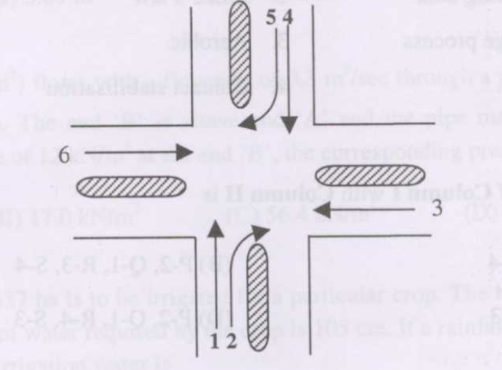
\includegraphics[width=0.5\linewidth]{figs/Q12.png}
	      \end{figure}
\begin{table}[h!]
  \centering
  \begin{tabular}[12pt]{ |c| c| c| c|}
    \hline
    \textbf{Combination choice} & \textbf{Phase I} & \textbf{Phase II} & \textbf{Phase III} \\ 
    \hline
    P & 1, 4 & 2, 5 & 3, 6 \\
    \hline 
    Q & 1, 2 & 4, 5 & 3, 6 \\
    \hline
    R & 2, 5 & 1, 3 & 4, 6 \\
    \hline
    S & 1, 4 & 2, 6 & 3, 5 \\
    \hline
    \end{tabular}

\end{table} 
\begin{enumerate}
    \item P
    \item Q
    \item R
    \item S \\
\end{enumerate}
			 \end{enumerate}
			 \end{document}
 
